% !TeX program = pdflatex
%
% Project Hive -- preprint
% Single-file: no external .bib required. Compile with:
%   pdflatex hive_preprint.tex   (twice, for cross-references)
%
\documentclass[11pt]{article}

\usepackage[margin=1in]{geometry}
\usepackage[T1]{fontenc}
\usepackage[utf8]{inputenc}
\usepackage{amsmath}
\usepackage{amssymb}
\usepackage{amsthm}
\usepackage{booktabs}
\usepackage{microtype}
\usepackage{algorithm}
\usepackage{algpseudocode}
\usepackage{tikz}
\usetikzlibrary{arrows.meta, positioning}
\usepackage[hidelinks]{hyperref}

\newtheorem{proposition}{Proposition}

\title{\textbf{Project Hive: A Resource-Bounded Multi-Agent Colony\\
over a Single Fine-Tuned 4B Language Model}}

\author{Arkapravo Pal\\
\small Independent Researcher\\
\small \texttt{arkapravopal04@gmail.com}}

\date{\today}

\begin{document}
\maketitle

\begin{abstract}
We describe Project Hive, a multi-agent system in which a single fine-tuned
4B-parameter language model is driven as a colony of specialised agents by a
non-model orchestrator that owns all state, scheduling, and lifecycle
decisions. The system takes one natural-language prompt, derives a complexity
tier and an energy budget from it, decomposes it into a dependency-gated task
graph, and returns a single natural-language answer; no human-readable text
crosses the system boundary in between. We propose four design commitments
that distinguish it from prompt-chaining approaches: (i) a strict separation
between latent reasoning (\texttt{think()}, raw single-token continuation over
a persistent key--value cache) and structured commitment (\texttt{decide()},
an independent constrained generation emitting exactly one action); (ii) a
complexity-derived energy budget that makes resource exhaustion a first-class,
recoverable terminal state rather than an unbounded loop; (iii) tiered
verification whose escalation cost is proportional to the stakes of the
decision being verified, with the firing tier reported so that expensive
verification can itself be charged against the budget; and (iv) a persistent
cross-session failure memory in which dead agents are distilled into
retrievable ``ghost'' records --- though we disclose in
Section~\ref{sec:failures} that a serialisation defect meant this mechanism
never once persisted a record in the runs we describe, so (iv) is a design we
argue for, not one we have evidence works. We give the architecture in full,
and we analyse the primitive that the next phase depends on: passing a
key--value cache between agents in place of text. We prove that under rotary
position embeddings a spliced cache with corrected position indices is
\emph{exactly} equal to the concatenated sequence, so that any measured
divergence is an implementation defect rather than information loss, and we
identify cache truncation as the sole point at which genuine approximation
enters. We report no quantitative task benchmarks; none of the four
commitments above, nor the complexity-scoring heuristic that gates every
downstream resource decision, has been validated against a baseline. We state
the evaluation protocol we intend to run, and we document the failure modes a
4B model exhibits inside structured agentic loops, several of which silently
disable entire subsystems.
\end{abstract}

\section{Introduction}
\label{sec:intro}

Much recent work described as ``multi-agent'' composes a small number of
language-model calls behind a prompt template. The composition is real, but the
resulting system has no state the orchestrator can inspect, no budget it can
exhaust, and no memory of what it already tried. Behaviour is obtained by
asking the model more carefully rather than by constraining what the system can
do.

Project Hive is an attempt at the opposite arrangement. A single model instance
is loaded once. Every agent is a thin reasoning wrapper around that shared
instance, holding its own key--value (KV) cache and its own role constraints.
Everything else --- who exists, what they are working on, what depends on what,
how much budget remains, who has failed and why --- lives in explicit data
structures owned by a non-model orchestrator. The model is asked to do exactly
one thing at a time and its output is parsed, verified, and accounted for
before it can affect the system.

The design target is deliberately austere: a single 16\,GB NVIDIA T4. That
constraint is not incidental. It forces every mechanism in the system to be
cheap enough to run alongside a resident 4B model, and it makes the number of
concurrent agents a function of available VRAM rather than of ambition.

\paragraph{Contributions.} The first three items below are architectural
claims, true by construction of the system we built; we do not yet have
evidence that any of them improves task outcomes relative to a baseline, and
we say so explicitly in Section~\ref{sec:eval}. Item 4 is weaker still: we
propose the mechanism, but as Section~\ref{sec:failures} discloses, it never
successfully persisted a record in the runs described here, so it is a design
argued for rather than one shown to work.
\begin{enumerate}
\item We propose an architecture in which latent reasoning and structured
      commitment are
      strictly separated at the level of the decoding loop, together with the
      empirical account of why the fused alternative failed
      (Section~\ref{sec:agent}).
\item We propose a complexity-to-budget derivation that converts a parsed
      problem specification into a scalar energy allowance, making resource
      exhaustion an explicit and recoverable terminal state (Sections~\ref{sec:phaser}
      and~\ref{sec:energy}); the derivation's coefficients are hand-set and
      unvalidated, as we note in Section~\ref{sec:phaser}.
\item We propose a three-tier verification scheme with cost-proportional
      escalation, in which the firing tier is reported to the caller so that
      the expensive tier can be charged against the same budget it consumes
      (Section~\ref{sec:judge}).
\item We propose a persistent failure memory that survives across sessions and
      is retrieved by task similarity, so that a respawned agent begins with a
      record of what has already failed on its task (Section~\ref{sec:ghosts});
      \textbf{disclosed in Section~\ref{sec:failures}: a serialisation defect
      meant this mechanism never once persisted a record in the runs we
      describe, so this contribution is unvalidated even qualitatively}.
\item We prove an exactness result for KV-cache splicing under rotary position
      embeddings, which localises the only genuine approximation in latent
      inter-agent communication to cache truncation
      (Section~\ref{sec:latent}).
\item A candid account of the failure modes a 4B model exhibits in structured
      agentic loops, including several that fail silently and disable whole
      subsystems (Section~\ref{sec:failures}).
\end{enumerate}

\section{Related Work}

\paragraph{Latent reasoning.}
Chain-of-thought prompting~\cite{wei2022cot} improved reasoning by having the
model externalise intermediate steps as tokens, at the cost of forcing all
intermediate computation through the discrete vocabulary bottleneck. Coconut
\cite{hao2024coconut} instead feeds the model's last hidden state directly back
as the next input embedding, allowing reasoning to proceed in continuous latent
space before any token is emitted. Our \texttt{think()} phase is a
resource-constrained variant of this idea: reasoning proceeds over a persistent
KV cache with no format expectations imposed on it, and commitment to a
structured action is deferred entirely to a separate call. LatentMAS
\cite{latentmas2025} extends latent reasoning across agents, exchanging
internal state rather than text. What we add beyond restating that goal is
narrowing where the actual design freedom lies: Proposition~\ref{prop:splice}
shows that position-corrected cache splicing is exact, which means the choice
of \emph{how much} of a producing agent's cache a consumer receives ---
truncation to the last $N$ entries, Section~\ref{sec:latent} --- is the one
open parameter, not the splicing mechanism itself. We treat that as the
pre-registered question our staged experiments (Section~\ref{sec:latent}) are
designed to answer, rather than a mechanism we still need to validate from
scratch.

\paragraph{Multi-agent frameworks.}
CAMEL~\cite{li2023camel}, AutoGen~\cite{wu2023autogen}, and
MetaGPT~\cite{hong2023metagpt} organise multiple language-model agents through
conversational protocols and assigned roles. These systems are considerably
more mature than ours in tooling and breadth. They differ in that
inter-agent communication is conversational, and agent population is
governed by the conversation rather than by an explicit resource budget. Hive
replaces the conversation with a typed event bus and an orchestrator-owned
dependency graph, and it caps the population with an energy economy.

\paragraph{Reflection and tool use.}
ReAct~\cite{yao2023react} interleaves reasoning traces with actions;
Reflexion~\cite{shinn2023reflexion} and Self-Refine~\cite{madaan2023selfrefine}
have a model revise its own output using verbal feedback;
Voyager~\cite{wang2023voyager} accumulates a reusable skill library across
episodes. Our ghost mechanism (Section~\ref{sec:ghosts}) is closest to
Reflexion, with two differences: the reflection is written by a separate
extraction step rather than by the failing agent itself, and it is persisted to
a vector index that outlives the session, so that a later run on a similar task
retrieves it. Toolformer~\cite{schick2023toolformer} established that models
can learn to invoke tools; our concern is narrower and operational, namely
containing what a tool call may do (Section~\ref{sec:tools}).

\paragraph{Efficient adaptation and inference.}
LoRA~\cite{hu2021lora} and QLoRA~\cite{dettmers2023qlora} make it feasible to
specialise a 4B model on a single consumer-class GPU, producing a
$\sim$50\,MB adapter rather than a duplicated model --- a prerequisite for
running the entire colony from one resident instance. Rotary position
embeddings~\cite{su2021rope} determine the correctness condition for cache
splicing in Section~\ref{sec:latent}, and grouped-query
attention~\cite{ainslie2023gqa} determines the per-token cache footprint that
bounds concurrency. Retrieval uses FAISS~\cite{johnson2017faiss} over
sentence embeddings~\cite{reimers2019sbert}.

\section{System Architecture}

\begin{figure}[t]
\centering
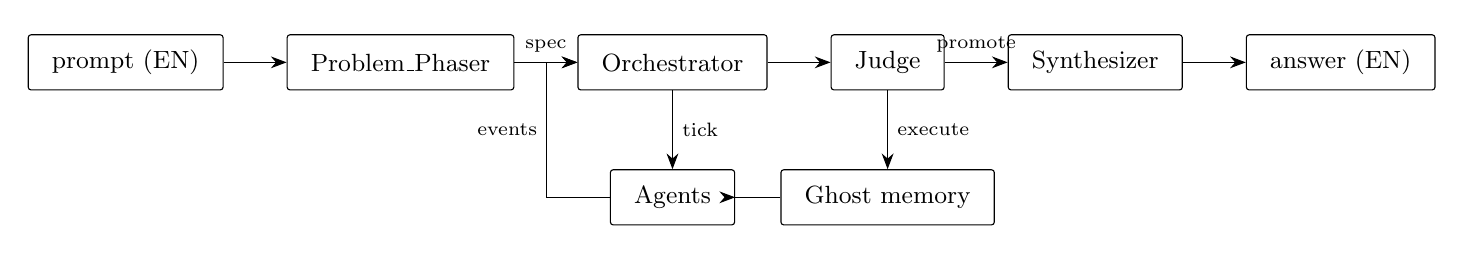
\begin{tikzpicture}[
  node distance=8mm,
  box/.style={draw, rounded corners=1pt, align=center, font=\small,
              minimum height=7mm, inner xsep=3mm},
  >={Stealth[length=2mm]}
]
\node[box] (in) {prompt (EN)};
\node[box, right=of in] (ph) {Problem\_Phaser};
\node[box, right=of ph] (orc) {Orchestrator};
\node[box, below=10mm of orc] (ag) {Agents};
\node[box, right=of orc] (jd) {Judge};
\node[box, below=10mm of jd] (gh) {Ghost memory};
\node[box, right=of jd] (sy) {Synthesizer};
\node[box, right=of sy] (out) {answer (EN)};

\draw[->] (in) -- (ph);
\draw[->] (ph) -- node[above, font=\scriptsize] {spec} (orc);
\draw[->] (orc) -- node[right, font=\scriptsize] {tick} (ag);
\draw[->] (ag.west) -- ++(-8mm,0) |- node[left, font=\scriptsize, pos=0.25] {events} (orc.west);
\draw[->] (orc) -- (jd);
\draw[->] (jd) -- node[right, font=\scriptsize] {execute} (gh);
\draw[->] (gh.west) -- ++(-6mm,0) -- (ag.east);
\draw[->] (jd) -- node[above, font=\scriptsize] {promote} (sy);
\draw[->] (sy) -- (out);
\end{tikzpicture}
\caption{System overview. Natural language crosses the system boundary exactly
twice --- the \emph{prompt (EN)} edge into Problem\_Phaser and the
\emph{answer (EN)} edge out of Synthesizer, the two leftmost and two
rightmost nodes above; every edge between them (spec, tick, events, execute,
promote) carries structured data, never free text. Agents never call the
orchestrator directly; they post typed events to a mailbox that the
orchestrator drains once per tick, which is the \emph{events} edge running
from Agents back to the Orchestrator.}
\label{fig:overview}
\end{figure}

\subsection{Problem phasing and budget derivation}
\label{sec:phaser}

The entry point performs four constrained extractions over the raw prompt:
the core objective, the situational background, an explicit requirement list,
and a domain classification in a fixed taxonomic format. Each is embedded with
a 384-dimensional sentence encoder~\cite{reimers2019sbert}. The result is a
specification dictionary, not prose; every downstream component consumes fields
of that dictionary rather than the original text.

A complexity score is then formed as the product of three independent signals.
Let $n$ be the number of extracted requirements, $d$ the macro-discipline of
the classified domain, and $g, c$ the goal and context embeddings. Then

\begin{align}
w_{\text{con}} &= \min\!\left(1.0 + 0.5\sqrt{n},\; 2.5\right), \\
w_{\text{sem}} &= 1.0 + 0.8\left(1 - \cos(g, c)\right), \\
S &= \mu(d)\cdot w_{\text{con}} \cdot w_{\text{sem}},
\end{align}

where $\mu(d)$ is a hand-assigned lookup table ranging from $1.0$ for general
discourse to $2.0$ for theoretical mathematics, interpolated linearly for
domains between (Table~\ref{tab:domain}).

\begin{table}[h]
\centering
\small
\begin{tabular}{@{}lc@{}}
\toprule
Domain (macro-discipline) & $\mu(d)$ \\
\midrule
Theoretical Mathematics & 2.0 \\
Aerospace \& Automation & 1.9 \\
Electrical \& Computer Engineering & 1.8 \\
Computer Science & 1.7 \\
Mechanical / Chemical Engineering & 1.6 \\
Finance \& Quantitative Analysis, Software Engineering & 1.5 \\
Biomedical \& Life Sciences & 1.4 \\
Data Engineering, Legal \& Compliance Analysis & 1.3 \\
Professional Communications, General Discourse & 1.0 \\
\bottomrule
\end{tabular}
\caption{Domain multiplier lookup table. An unmatched classification falls
back to substring match against these keys, then to $1.0$.}
\label{tab:domain}
\end{table}

The constraint term uses a square-root curve because the marginal difficulty
of an additional constraint diminishes: the tenth requirement in a
specification rarely costs what the second did. The semantic term penalises
specifications whose stated goal is distant from their stated context, on the
assumption that such a gap indicates work the prompt has left implicit.

We state plainly what Eqs.~1--3 are and are not. Every constant in them ---
the $0.5$ and $2.5$ in $w_{\text{con}}$, the $0.8$ in $w_{\text{sem}}$, every
entry of $\mu(d)$, the choice of $\sqrt{n}$ over $\log n$ or $n^{0.4}$ --- is
hand-set to match our intuition about relative difficulty, not fit to data or
validated against an outcome. We have not run a sensitivity analysis, and we
have not shown that the resulting score tracks difficulty better than a flat
budget would. This matters more than a typical hyperparameter choice because
$S$ gates every downstream resource decision --- tier, energy budget, and
therefore how much of the architecture in the rest of this section is even
exercised for a given problem. We list it as an ablation target in
Section~\ref{sec:eval} (flat budget in place of the complexity-derived one)
precisely because we regard it as unvalidated, not because we expect it to
survive unchanged.

$S$ is clamped to $[1.0, 9.0]$ and mapped by piecewise-linear interpolation
across five anchors onto an energy budget in $[100, 3000]$, with tier
boundaries at $S \le 2.0$ (S), $S \le 3.5$ (M), $S \le 6.0$ (L), and above (XL).
Interpolation rather than a per-tier constant is deliberate: a problem sitting
just above a tier boundary should not receive an allowance discontinuously
larger than one sitting just below it. The death and stress thresholds that
this budget is eventually spent down to
($\theta_{\text{death}}=5$, $\theta_{\text{stress}}=10$, Section~\ref{sec:energy})
are fixed constants independent of tier: against an S-tier budget of $100$
they represent exhausting $95$--$90\%$ of the allowance, but against an
XL-tier budget of $3000$ they represent $99.7$--$99.8\%$. We have not verified
that ``5 energy remaining'' is an equivalently meaningful stopping point across
tiers, and it plausibly is not --- a fixed absolute threshold on a budget that
itself spans $100$--$3000$ is another unvalidated design choice, structurally
similar to the one above.

\subsection{Task graph and event bus}

Work is represented as a directed acyclic graph of task nodes carrying a
description, a status in $\{$pending, running, complete, failed$\}$, a
dependency list, an in-degree, an assigned agent, and a result slot. Completing
a task decrements the in-degree of its dependents and returns those that reach
zero. Failing a task marks its entire transitive dependent closure as failed;
there is no partial credit downstream of a failure. Cycle introduction is
detected at insertion time by breadth-first search over the dependents of the
new node, and reported immediately --- an undetected cycle would otherwise
leave the colony ticking indefinitely with no diagnostic, since no node in the
cycle can ever reach in-degree zero.

Agents do not invoke the orchestrator. They append typed events ---
\texttt{spawn\_request}, \texttt{completion\_request}, \texttt{failure\_request},
\texttt{tool\_request}, \texttt{parent\_notification} --- to a mailbox that the
orchestrator drains exactly once per tick. This single choke point is what
makes colony state legible at any instant, and it is a prerequisite for the
latent-communication work in Section~\ref{sec:latent}: replacing the payload of
an event is a local change, whereas replacing the arguments of a direct call
would not be.

\subsection{The orchestrator loop}

\begin{algorithm}[t]
\caption{\textsc{Tick} --- one heartbeat of the colony}
\label{alg:tick}
\begin{algorithmic}[1]
\State $e \gets$ remaining energy
\If{$e \le \theta_{\text{death}}$} \State \Return \textsc{Halt} \Comment{terminal: energy death}
\ElsIf{$e \le \theta_{\text{stress}}$} \State \Call{Consolidate}{} \Comment{attempt to reclaim}
\EndIf
\State \Call{DeadlockWatchdog}{} \Comment{scaled-timeout liveness check}
\State $E \gets$ \Call{Drain}{mailbox}; \Call{Route}{$E$}
\State \Call{DispatchUnblocked}{} \Comment{tasks whose in-degree reached zero}
\State \Call{TickLiveAgents}{} \Comment{think / decide / execute}
\If{root task is complete} \State \Return \textsc{Halt} \Comment{terminal: success}
\EndIf
\State \Return \textsc{Continue}
\end{algorithmic}
\end{algorithm}

The order in Algorithm~\ref{alg:tick} is load-bearing. State is settled before
any agent is allowed to move: energy is evaluated against a snapshot, liveness
is checked before new work is admitted, the mailbox is drained to quiescence,
and only then are agents ticked. Interleaving these --- in particular, ticking
agents while the mailbox still holds unrouted events --- makes the colony's
observable state depend on iteration order over a dictionary.

The deadlock watchdog scales its timeout by the number of currently tickable
agents. A fixed timeout is wrong here for a mechanical reason: agents share one
model instance and are ticked sequentially, so the wall-clock silence of any
individual agent grows linearly with the number of its peers. A fixed threshold
would therefore begin killing healthy agents precisely as the colony became
busy.

\subsection{The agent cognitive cycle}
\label{sec:agent}

Each agent alternates three phases.

\paragraph{\texttt{think()}.}
The model is invoked directly --- not through a generation wrapper --- with a
persistent \texttt{past\_key\_values}, one token at a time, greedily, feeding
its own last token back as the next input. There are no stop strings, no format
instructions, and no expectation that anything parseable will emerge. Emission
is capped per cycle by role (decomposer 128, executor 256, verifier 128 tokens)
against a hard lifetime ceiling of $4096$ tokens per agent, which is also the
figure that bounds per-agent cache footprint.

\paragraph{\texttt{decide()}.}
A separate, independent generation from a freshly constructed prompt. It emits
exactly one action from $\{$\textsc{think}, \textsc{spawn}, \textsc{tool},
\textsc{report}, \textsc{die}$\}$ together with a payload, in an
\texttt{ACTION:}/\texttt{PAYLOAD:} format. Parsing is layered: a labelled
match, then a bare leading keyword, then trailing-brace trimming for truncated
JSON, then Python literal evaluation for single-quoted dictionaries. Generation
is retried up to three times with sampling enabled if the output is detected as
degenerate.

\paragraph{\texttt{execute()}.}
The committed action is converted into a typed event and posted to the mailbox.

The separation between the first two phases is the central architectural claim
of this work, and it was arrived at by failure. Earlier revisions had
\texttt{think()} monitor its own output stream for action keywords and exit
early when one appeared, on the intuition that this would save a redundant
call. It did the opposite. Given a token budget intended for open-ended
reasoning, the model raced to produce a well-formed decision inside it,
truncating the reasoning that the budget existed to permit. Worse, the saving
was illusory: \texttt{decide()} was invoked afterwards regardless of how
\texttt{think()} exited. Enforcing the separation --- \texttt{think()} never
produces a decision, \texttt{decide()} never reasons open-endedly --- resolved
both. The resulting boundary is the latent-space analogue of the distinction
between a reasoning trace and a tool call in text-level agent
frameworks~\cite{yao2023react}.

\subsection{Tiered verification}
\label{sec:judge}

No result reaches its parent unverified. Verification escalates in three tiers
whose costs differ by orders of magnitude (Table~\ref{tab:tiers}).

\begin{table}[t]
\centering
\begin{tabular}{@{}llll@{}}
\toprule
Tier & Check & Cost & Runs when \\
\midrule
1 & syntax, shape, emptiness              & sub-millisecond    & always \\
2 & cosine similarity to goal embedding   & one dot product    & output embedding computed \emph{and} $>$12 words \\
3 & language-model critique of engagement & a full generation  & agent is attempting promotion \\
\bottomrule
\end{tabular}
\caption{Verification tiers. The verdict returned to the orchestrator names the
tier that produced it, so that tier-3 consumption can be charged against the
energy budget. Tier 2's condition is two independent gates, not one, and in
the system as \texttt{main.py} constructs it, with every component injected,
only the second ever actually fires: the goal embedding is computed once per
prompt during phasing
and the shared embedder is always injected, so both are present on every run
that has a phaser configured at all; the length gate is the one that
determines, per output, whether tier 2 runs. The ``embedding present'' gate
still exists structurally --- it protects a caller that constructs the
orchestrator without a phaser or embedder, as some of our own tests do --- but
readers should not expect to observe it firing in a normal run. We list both
gates explicitly here rather than the single ``when embeddings exist''
condition an earlier draft of this table used, which conflated the two.}
\label{tab:tiers}
\end{table}

Tier 2 issues one of three verdicts by similarity $s$ between the output
embedding and the colony goal embedding: $s \le 0.30$ is fatal and the agent is
terminated; $s \le 0.60$ produces a warning, with a correction written directly
into the agent's failure-reason field so that it appears in the next prompt;
three accumulated warnings terminate the agent. Outputs shorter than twelve
words bypass tier 2 entirely rather than be judged by a similarity score that
carries no signal at that length --- a terse correct answer and a terse wrong
answer are equally distant from a goal embedding.

Tier 3 is reserved for the single moment it matters, the attempt to promote a
result to a parent, and asks whether the agent engaged with the problem as
posed or silently substituted an easier one. Because tier 3 is a full
generation occurring outside any agent's own reasoning loop, its cost is
invisible to the per-agent accounting described in Section~\ref{sec:energy};
returning the firing tier alongside the verdict is what allows the orchestrator
to charge for it.

\subsection{Failure memory}
\label{sec:ghosts}

When an agent is terminated, a \emph{ghost} record is extracted before its
state is released: role, task, a failure type in $\{$self-reported,
semantic-drift, tier-1 crash$\}$, the failure reason, accumulated warnings,
thought process, and energy consumed. The record is embedded and written to a
FAISS inner-product index~\cite{johnson2017faiss} that is persisted to disk and
reloaded on subsequent sessions. A newly spawned agent queries the index by its
own task description and receives the nearest ghosts as context before it
begins reasoning. A second index caches successful subtask results above a
$0.45$ similarity threshold; it is session-scoped and never written to disk,
since a cached success is only sound within the specification that produced it.

Failure reasons are deduplicated and length-capped before storage. This is not
cosmetic: under greedy decoding a small model's self-reported termination
reason frequently degenerates into the same clause repeated many times, and
storing that verbatim both wastes index space and produces a retrieved context
that crowds out the prompt it was meant to inform.

\subsection{Energy economy}
\label{sec:energy}

A terminological note before the mechanics: we use \emph{energy} for the
single decrementing scalar counter defined below, \emph{budget} for its
initial value (Section~\ref{sec:phaser}'s $S \to [100,3000]$ mapping), and
\emph{economy} loosely, for the debit/threshold/consolidation system as a
whole rather than as a claim that a market, price signal, or exchange
mechanism is present --- there is no such mechanism in Phase~1, and
``economy'' should be read as a design metaphor, not a technical term
introducing new machinery beyond the counter and its two thresholds.
\emph{Tier} (S/M/L/XL) is a discrete band of $S$ used only to select a point
on that interpolation and plays no further role once the budget is set.

A single scalar budget, initialised from Section~\ref{sec:phaser}, is debited
on two events: agent creation (decomposer 4, executor 2, verifier 2) and
reasoning, at $\max(1, \lfloor \Delta c / 100 \rfloor)$ per agent per tick,
where $\Delta c$ is the growth in that agent's accumulated thought text. Below
$\theta_{\text{stress}} = 10$ the colony attempts consolidation; at or below
$\theta_{\text{death}} = 5$ it halts and returns the best partial synthesis it
can assemble from completed subtasks, explicitly labelled as partial.

Two properties of this design are worth stating. First, energy exhaustion is a
\emph{recoverable} terminal state, not a crash: the system is required to
produce an answer from whatever completed, and to say plainly that it did so
under exhaustion. Second, the budget is not what bounds concurrency. Fan-out is
capped structurally and independently at three subtasks from the root and two
from any other agent, and it is that cap --- not the budget --- that bounds the
number of simultaneously resident KV caches. Section~\ref{sec:latent} explains
why this distinction becomes critical.

\subsection{Sandboxed tool use}
\label{sec:tools}

Five tools (code execution, symbolic and computational mathematics, tabular
query, file read, file write) are routed through a single dispatcher behind an
eight-way concurrency semaphore. Agent-supplied code executes in a subprocess
under stacked restrictions: network gating, process-spawn gating, module-import
gating, address-space and CPU-time resource limits, path jails confining reads
and writes to dedicated temporary roots, byte caps on captured output, and a
timeout clamped to $[1, 120]$ seconds before per-domain scaling. Tool
availability is domain-conditional; legal and compliance work cannot invoke
code execution at all.

The timeout clamp is a direct consequence of an incident. An agent-supplied
timeout previously flowed unvalidated into the subprocess call and was
multiplied by the domain scale; a single runaway script consequently ran for
approximately eleven days before external termination. The general lesson is
that any numeric parameter a language model can emit must be validated against
a hard range at the boundary, since the model has no notion of the units it is
choosing in.

\subsection{Synthesis}

On completion, all finished task results are gathered in dependency order by a
topological walk and combined by exactly one generation into a single answer
addressed to the original problem. This is the only point at which the system
composes prose for a human. Conflict resolution across agents attempting the
same subtask is not required in the present phase, since no two agents are
assigned identical work; the interface for it exists and is the only component
that changes if that invariant is relaxed.

\section{Toward Latent Inter-Agent Communication}
\label{sec:latent}

Agents currently communicate by text: a completing agent's result is decoded to
a string, and a dependent agent receives a truncated tail of it re-tokenised
into a fresh prompt. This is lossy twice over --- once at truncation, once at
the decode/re-encode boundary --- and it discards the attention state that
produced the result. The alternative, following LatentMAS
\cite{latentmas2025}, is to make the producing agent's KV cache a prefix of the
consuming agent's context. Before adopting it we establish what it costs and
what it preserves.

\subsection{Exactness of position-corrected splicing}

Rotary position embeddings~\cite{su2021rope} apply a position-dependent
rotation to queries and keys at the time they are computed. For a token at
position $i$ in layer $\ell$, the cached entries are
$k_i^{(\ell)} = R_{\Theta,i} W_K x_i^{(\ell)}$ and
$v_i^{(\ell)} = W_V x_i^{(\ell)}$, and the attention logit between a query at
position $j$ and that key is
\begin{equation}
\langle R_{\Theta,j} W_Q x_j,\; R_{\Theta,i} W_K x_i \rangle
= \langle W_Q x_j,\; R_{\Theta,\,j-i} W_K x_i \rangle ,
\label{eq:rope}
\end{equation}
which depends on $i$ and $j$ only through their difference.

\begin{proposition}
\label{prop:splice}
Let agent $A$ have consumed tokens $a_0,\dots,a_{P-1}$ at positions
$0,\dots,P-1$, producing cache $C_A$, and let agent $B$ have tokens
$b_0,\dots,b_{M-1}$. Running $B$ with \texttt{past\_key\_values} $= C_A$ and
position indices $P,\dots,P+M-1$ yields, for every layer and every token of
$B$, exactly the hidden states obtained by running the concatenated sequence
$a \Vert b$ in a single forward pass, up to floating-point non-associativity.
\end{proposition}

\begin{proof}
By induction on layers $\ell = 0, 1, \dots$. At $\ell = 0$, $B$'s inputs are its
own token embeddings $x_{b_t}^{(0)}$ in both settings, since embedding lookup
does not depend on position. Assume the inductive hypothesis: for every
$t = 0,\dots,M-1$, $B$'s layer-$\ell$ input $x_t^{(\ell)}$ (writing $x_t$ for
$x_{b_t}$) is identical bit-for-bit between the spliced and concatenated runs.
We show the layer-$\ell$ attention sublayer then produces identical outputs,
which are $B$'s layer-$(\ell{+}1)$ inputs, closing the induction.

Fix a query at $B$'s position $t$ (absolute position $P+t$ in both settings).
Let $I_t = \{0,\dots,P-1\} \cup \{0,\dots,t\}$ index, respectively, the $P$
tokens of $A$ and the first $t{+}1$ tokens of $B$ --- i.e.\ every key this
query may attend to under the causal mask. This index set is the same object
in both settings: the concatenated pass masks to positions $\{0,\dots,P+t\}$ of
one sequence, which are exactly $a_0,\dots,a_{P-1},b_0,\dots,b_t$; the spliced
pass masks to $C_A$'s $P$ cached entries plus the $t{+}1$ entries $B$ has
written into the cache so far, which are the same $P{+}t{+}1$ tokens by
construction. So the two settings sum over identical key/value \emph{sets}, not
merely sets of equal size --- this is the fact the induction hypothesis and the
cache-construction give us for free, and it is what licenses comparing the
softmax outputs term-by-term next.

For each $i \in I_t$, write $k_i, v_i$ for the key and value vectors token $i$
contributes. By the inductive hypothesis (for $i$ a token of $B$) or by
construction of $C_A$ (for $i$ a token of $A$, cached once and never
recomputed), $x_i^{(\ell)}$ --- and hence $k_i = W_K x_i^{(\ell)}$ and
$v_i = W_V x_i^{(\ell)}$ before rotation --- is identical in both settings.
Rotation is applied at the position each token actually occupies: $A$'s tokens
carry rotation angles for $0,\dots,P-1$ and $B$'s carry rotation angles for
$P,\dots,P+t$ in \emph{both} settings, by hypothesis in the concatenated case
and by explicit construction (\texttt{position\_ids} $= P,\dots,P+M-1$) in the
spliced case. So the rotated key $R_{\Theta,i}k_i$ agrees for every
$i \in I_t$, and by \eqref{eq:rope} every logit
$\ell_i = \langle W_Q x_t^{(\ell)}, R_{\Theta,\,(P+t)-i}\,k_i\rangle$ agrees for
every $i \in I_t$ as well, since it depends only on the identical query, the
identical rotated key, and the relative offset $(P+t)-i$, which is the same
number in both settings regardless of how the underlying cache is stored.

The two settings therefore compute
$\operatorname{softmax}_{i \in I_t}(\ell_i)$ over the \emph{same finite
multiset} of real numbers $\{\ell_i\}_{i \in I_t}$: same index set (previous
paragraph), same value at each index (this paragraph). Softmax is a function
of its input vector alone, so the resulting attention weights $\alpha_i$ are
identical, term for term, in both settings --- this is the normalisation step
the proof sketch in an earlier draft of this result asserted without stating;
it holds because the two prior facts (identical index set, identical per-index
logit) are exactly what softmax needs as input, and nothing else. The value
vectors $v_i$ are unrotated and already shown identical, so the attention
output $\sum_{i \in I_t} \alpha_i v_i$ is identical, and after the identical
output projection $W_O$, so is $x_t^{(\ell+1)}$. This holds for every
$t = 0,\dots,M-1$ simultaneously, completing the inductive step.
\end{proof}

\paragraph{Applicability to grouped-query attention.} The model this system
targets uses GQA~\cite{ainslie2023gqa}, in which multiple query heads within a
group share one key/value head rather than each query head owning its own.
The proof above goes through unchanged under GQA, because nothing in it
depends on the number of query heads per key/value head: fix a KV-head group,
and the argument is stated entirely in terms of \emph{that group's} $k_i, v_i$
and the query heads that read them, with rotation, caching, and position
indexing all happening at the granularity of the shared key/value projection,
not the query head. Running the same argument once per KV-head group covers
every query head, since each query head within a group is just a different
$W_Q$ applied to the same shared keys and values under the same index set
$I_t$ and the same rotation angles. GQA changes cache \emph{size} (via the
key/value head count, relevant to the cache-census experiment below) but
introduces no new term into \eqref{eq:rope} or into the softmax argument
above, so exactness is unaffected.

Proposition~\ref{prop:splice} has a practical consequence that shaped our
experimental design: a nonzero divergence between position-corrected splicing
and the concatenated reference is evidence of a defect in the implementation,
not evidence that latent transfer is lossy. Splicing without position
correction --- leaving $B$'s tokens at $0,\dots,M-1$ atop a $P$-token cache ---
is the failure this predicts, and it is a dangerous one, because it raises no
exception. Two distinct tokens claim each position, every relative offset in
\eqref{eq:rope} is wrong by $P$, and the model emits fluent, plausible, wrong
output.

\subsection{Where approximation genuinely enters}

Transmitting a full 4096-token cache per inter-agent message defeats the
purpose of avoiding text. The operative question is therefore what survives
truncation to the last $N$ entries of $C_A$. Under truncation
Proposition~\ref{prop:splice} no longer applies: $B$ attends over a strict
subset of the keys the concatenated sequence would offer, and real information
is lost. This --- not position handling --- is the design question, and it is
the one our experiments are constructed to answer.

\subsection{Experimental protocol}

Three staged experiments gate this work; each one's outcome determines whether
the next is worth running.

\begin{enumerate}
\item \textbf{Cache census.} Measure realised KV bytes per token with the model
      resident, and derive how many concurrent agent caches fit in remaining
      VRAM at the 4096-token ceiling. The config-derived figure must use the
      grouped-query key/value head count~\cite{ainslie2023gqa} rather than the
      attention head count; the latter overstates the cache by the grouping
      ratio. A GPU--CPU round trip for one full cache is timed to establish
      whether eviction is viable or whether concurrency must simply be capped.
\item \textbf{Reasoning-to-decision bridge.} Compare the current arrangement,
      in which \texttt{decide()} rebuilds a prompt containing a truncated tail
      of the reasoning, against appending \texttt{decide()}'s instruction
      tokens directly to \texttt{think()}'s cache. Metrics are format
      compliance and prefix tokens saved per decision. This requires no
      training and is the immediately shippable change; it also requires
      crop-based rewind, since generating on a shared cache mutates it and a
      retry would otherwise build on its own failed attempt.
\item \textbf{Cache splice.} Five arms --- $B$ alone (floor), concatenated
      reference (ceiling, GOLD), naive splice, position-corrected splice, and
      truncated splice --- compared by Kullback--Leibler divergence of the
      next-token distribution against the reference, plus top-1 and top-5
      agreement. We report the \emph{forward} direction,
      $D_{\mathrm{KL}}(P_{\mathrm{GOLD}} \,\|\, P_{\mathrm{arm}})$, not the
      reverse. KL is asymmetric and the two directions answer different
      questions: forward KL is mode-covering and is large whenever GOLD places
      non-trivial mass on a continuation the arm assigns near-zero probability
      to, i.e.\ it penalises an arm for \emph{failing to preserve} something
      the fully-informed reference would say. Reverse KL is mode-seeking and
      would instead penalise an arm for hallucinating mass GOLD does not have,
      while tolerating an arm that confidently collapses onto one of several
      continuations GOLD considered live. Since the question this experiment
      exists to answer is whether a spliced or truncated cache \emph{loses}
      information relative to the full concatenated context, forward KL is the
      direction that measures loss; reverse KL would systematically understate
      it. Divergence rather than output text: two arms can produce identical
      greedy output while sitting on materially different distributions, and
      that difference only surfaces later under sampling or over a longer
      horizon. The reference must be constructed by token-level concatenation
      rather than by joining strings and re-tokenising, since a re-tokenised
      seam yields a different token sequence and would place an irreducible
      floor under every measured divergence.
\end{enumerate}

\section{Failure Modes of Small Models in Structured Loops}
\label{sec:failures}

A 4B model in an agentic loop fails in ways that are specific enough to be
worth cataloguing, and several of them are silent. \textbf{A note on evidence
before we do:} every failure below was observed at least once during
development and is real, but none was measured for frequency across repeated
trials. We report them as documented single-occurrence (or few-occurrence)
observations that motivated a specific fix, not as rates, and we flag each
one's evidentiary status inline rather than let the catalogue format imply
otherwise.

\paragraph{Degenerate greedy decoding.} With sampling disabled and no
repetition penalty, generation reliably enters verbatim sentence-level loops
once it exhausts substantive content. \emph{Single documented occurrence:} we
observed one synthesis output repeat the same sentence fourteen times; we have
not measured how often this recurs across runs. A per-token repetition penalty alone is
insufficient, because it discounts tokens cumulatively and does not reliably
block a multi-word phrase whose individual tokens are common elsewhere in a
long prompt; an $n$-gram repetition block addresses the phrase-level case more
directly.

\paragraph{Repetition penalties corrupting required repetition.} \emph{Single
documented occurrence, not a measured rate.} The converse
error is instructive. A repetition penalty strong enough to suppress looping
(1.3) caused the verification critic to avoid re-emitting the literal tokens
of its own verdict keywords, fragmenting them into oddly spaced subwords that
the verdict parser could not match --- silently discarding what may have been
the model's actual determination. Any prompt that structurally requires a
keyword to recur constrains how aggressive the penalty may be.

\paragraph{Fail-closed defaults compounding parse brittleness.} The critic
defaulted to rejection when no verdict line could be parsed. Combined with a
strict line-initial parse that a small model does not reliably satisfy, this
produced deterministic rejection on every attempt. Because decoding was greedy,
every respawn reproduced the identical failure, and the colony consumed its
entire budget on an unchanging loop. A fail-closed default is correct in
isolation and catastrophic when paired with a brittle parser and a
deterministic retry.

\paragraph{Order-sensitivity in verdict extraction.} A small model asked to
critique its own work commonly narrates through a correction, emitting a
rejection and then revising to acceptance within the same response. Taking the
first verdict encountered locks in a draft the model itself has already
withdrawn; the last verdict is the one it concluded with.

\paragraph{Empty generations.} When the padding token equals the
end-of-sequence token and no minimum-length floor is set, greedy decoding emits
end-of-sequence as its very first token on certain prompt shapes, yielding an
empty string that propagates downstream as a successfully completed but
contentless result.

\paragraph{Silent subsystem loss.} \textbf{This is the most consequential item
in this catalogue, not the last one; it is placed here only to keep the
catalogue's ordering by failure category, and we repeat it in the abstract and
in contribution~4 of Section~\ref{sec:intro} for that reason.} The most
consequential failures were not model failures. Exception handlers around
persistence calls converted genuine errors into no-ops: a GPU tensor leaking
into a supposedly JSON-serialisable ghost record caused every write to fail
silently, so the failure memory had never once persisted despite appearing to
function in every session we ran before this was found. Concretely: the ghost
mechanism described in Section~\ref{sec:ghosts} and claimed as contribution~4
was, for every run predating this fix, decorative --- it executed, logged
nothing suspicious, and returned control normally, while contributing zero
retrievable records to the index it was writing to. We note this because it
generalises beyond this one bug --- in a system where subsystems are invoked
opportunistically and wrapped defensively, an unavailable subsystem is
observationally indistinguishable from an idle one, which is precisely why we
regard contribution~4 as unvalidated rather than merely under-evaluated.

\section{Evaluation Protocol}
\label{sec:eval}

We report no quantitative task benchmarks in this preprint. The system is
functional end to end --- it decomposes, delegates, verifies, recovers from
failure, and answers --- but we regard reporting numbers before the protocol
below has been run as premature, particularly given that
Section~\ref{sec:failures} documents subsystems that appeared functional while
being disabled. We state the protocol so that it can be criticised before
rather than after it produces results.

\paragraph{Task suites.} Multi-constraint engineering design problems spanning
the domain taxonomy, at each of the four complexity tiers, with a
single-agent chain-of-thought baseline on the identical model and adapter. We
intend at least 15 problems per tier (60 total), each run under 3 seeds to
give a within-condition spread rather than a single point estimate; this is a
target we have not yet met, and we state it here specifically so it can be
checked against what is eventually reported.

\paragraph{Decoding.} All conditions --- Hive and the baseline --- use the same
generation settings the rest of this paper describes (greedy for
\texttt{think()}/synthesis, the layered retry-with-sampling only inside
\texttt{decide()} on detected degeneration). We do not evaluate under a
sampled-decoding regime in this protocol: greedy decoding is deterministic
given fixed weights, so a report of ``answer quality'' under it is exactly
reproducible from the same model and adapter, at the cost of not
characterising variance a sampled deployment would actually see. This is a
scope limitation of the protocol, not evidence that the system's behaviour
under sampling is equivalent.

\paragraph{Primary metrics.} (i) End-to-end answer quality under blind
comparison against the baseline; (ii) constraint satisfaction rate, measured
against the requirement list the phaser extracted, which gives a checkable
per-constraint ground truth without requiring a reference answer; (iii) energy
consumed per solved problem, and the fraction of runs terminating in energy
death rather than success.

\paragraph{Ablations.} Each mechanism removed independently: no ghost
retrieval; verification truncated to tier 1; fused \texttt{think()}/%
\texttt{decide()}; flat budget in place of the complexity-derived one; base
model in place of the adapter. The first and third are the claims most in need
of falsification --- respectively, that persisted failure memory improves
subsequent attempts, and that separating latent reasoning from structured
commitment outperforms fusing them.

\paragraph{Latent-communication metrics.} As specified in
Section~\ref{sec:latent}, reported as distributional divergence against a
token-level concatenated reference, with the truncation sweep reported as a
curve in $N$ rather than at a single operating point.

\section{Limitations}

Inter-agent communication remains textual; the latent path is analysed here but
not yet integrated. Sibling dependencies within a single spawn decision are not
addressable --- the task graph gates on dependencies correctly, but an agent
cannot name a peer's task identifier in the decision that creates them both, so
in practice dependency structure is shallower than the graph permits. The
energy economy is a single flat currency; the two-currency design we intended,
separating compute from confidence-debt, is not built, and consequently an
agent cannot be made to pay more for asserting something it is unsure of. The
consolidation mechanism invoked under energy stress is presently inert, since
no code path assigns the idle status it searches for, leaving the fan-out cap
as the only functioning population control. Results are reported from a single
model at a single scale on a single GPU; nothing here establishes how these
mechanisms behave at larger scale, where several of them --- the energy economy
and the tiered critic in particular --- exist principally to compensate for
limited model capability.

\section{Conclusion}

Project Hive treats a language model as a component to be scheduled rather than
a system to be prompted. The orchestrator owns state, budget, and lifecycle;
the model reasons and commits, one action at a time, into a structure that
validates and accounts for what it produced. The mechanisms that make this
work at 4B scale on one GPU --- strict separation of latent reasoning from
structured commitment, an energy budget derived from measured problem
complexity, verification whose cost scales with the stakes of the decision, and
a failure memory that outlives the session --- are individually modest, and are
reported here alongside the failures that motivated each of them. The exactness
result of Section~\ref{sec:latent} indicates that the transition to latent
inter-agent communication is a plumbing problem with one genuine design
question inside it, namely how much of a producing agent's attention state a
consumer actually requires. That question, and the evaluation protocol of
Section~\ref{sec:eval}, are the immediate next work.

\paragraph{Availability.} Source is available at
\url{https://github.com/arkapravopal04/Swarm_neural_nets}.

\begin{thebibliography}{99}
\small

\bibitem{ainslie2023gqa}
J.~Ainslie, J.~Lee-Thorp, M.~de~Jong, Y.~Zemlyanskiy, F.~Lebrón, and S.~Sanghai.
\newblock GQA: Training generalized multi-query transformer models from
  multi-head checkpoints.
\newblock \emph{arXiv:2305.13245}, 2023.

\bibitem{dettmers2023qlora}
T.~Dettmers, A.~Pagnoni, A.~Holtzman, and L.~Zettlemoyer.
\newblock QLoRA: Efficient finetuning of quantized LLMs.
\newblock \emph{arXiv:2305.14314}, 2023.

\bibitem{hao2024coconut}
S.~Hao, S.~Sukhbaatar, D.~Su, X.~Li, Z.~Hu, J.~Weston, and Y.~Tian.
\newblock Training large language models to reason in a continuous latent space.
\newblock \emph{arXiv:2412.06769}, 2024.

\bibitem{hong2023metagpt}
S.~Hong, X.~Zheng, J.~Chen, et~al.
\newblock MetaGPT: Meta programming for multi-agent collaborative framework.
\newblock \emph{arXiv:2308.00352}, 2023.

\bibitem{hu2021lora}
E.~J. Hu, Y.~Shen, P.~Wallis, Z.~Allen-Zhu, Y.~Li, S.~Wang, L.~Wang, and
  W.~Chen.
\newblock LoRA: Low-rank adaptation of large language models.
\newblock \emph{arXiv:2106.09685}, 2021.

\bibitem{johnson2017faiss}
J.~Johnson, M.~Douze, and H.~Jégou.
\newblock Billion-scale similarity search with GPUs.
\newblock \emph{arXiv:1702.08734}, 2017.

\bibitem{latentmas2025}
LatentMAS: Latent-space multi-agent systems.
\newblock \emph{arXiv:2511.20639}, 2025.

\bibitem{li2023camel}
G.~Li, H.~A.~A.~K. Hammoud, H.~Itani, D.~Khizbullin, and B.~Ghanem.
\newblock CAMEL: Communicative agents for ``mind'' exploration of large language
  model society.
\newblock \emph{arXiv:2303.17760}, 2023.

\bibitem{madaan2023selfrefine}
A.~Madaan, N.~Tandon, P.~Gupta, et~al.
\newblock Self-Refine: Iterative refinement with self-feedback.
\newblock \emph{arXiv:2303.17651}, 2023.

\bibitem{reimers2019sbert}
N.~Reimers and I.~Gurevych.
\newblock Sentence-BERT: Sentence embeddings using Siamese BERT-networks.
\newblock \emph{arXiv:1908.10084}, 2019.

\bibitem{schick2023toolformer}
T.~Schick, J.~Dwivedi-Yu, R.~Dessì, et~al.
\newblock Toolformer: Language models can teach themselves to use tools.
\newblock \emph{arXiv:2302.04761}, 2023.

\bibitem{shinn2023reflexion}
N.~Shinn, F.~Cassano, E.~Berman, A.~Gopinath, K.~Narasimhan, and S.~Yao.
\newblock Reflexion: Language agents with verbal reinforcement learning.
\newblock \emph{arXiv:2303.11366}, 2023.

\bibitem{su2021rope}
J.~Su, Y.~Lu, S.~Pan, A.~Murtadha, B.~Wen, and Y.~Liu.
\newblock RoFormer: Enhanced transformer with rotary position embedding.
\newblock \emph{arXiv:2104.09864}, 2021.

\bibitem{wang2023voyager}
G.~Wang, Y.~Xie, Y.~Jiang, et~al.
\newblock Voyager: An open-ended embodied agent with large language models.
\newblock \emph{arXiv:2305.16291}, 2023.

\bibitem{wei2022cot}
J.~Wei, X.~Wang, D.~Schuurmans, et~al.
\newblock Chain-of-thought prompting elicits reasoning in large language models.
\newblock \emph{arXiv:2201.11903}, 2022.

\bibitem{wu2023autogen}
Q.~Wu, G.~Bansal, J.~Zhang, et~al.
\newblock AutoGen: Enabling next-gen LLM applications via multi-agent
  conversation.
\newblock \emph{arXiv:2308.08155}, 2023.

\bibitem{yao2023react}
S.~Yao, J.~Zhao, D.~Yu, N.~Du, I.~Shafran, K.~Narasimhan, and Y.~Cao.
\newblock ReAct: Synergizing reasoning and acting in language models.
\newblock \emph{arXiv:2210.03629}, 2022.

\end{thebibliography}

\end{document}
